\begin{figure}[H]
    \centering

    \tikzset{
    max/.style={circle,draw,inner sep=5},
    min/.style={circle,draw,inner sep=5, fill=gray},
    bold/.style={line width=1mm},
    thin/.style={line width=0.2mm}
    }

    % Specify spacing for each level of the tree
    \tikzstyle{level 1}=[level distance=1mm,sibling distance=2mm]
    \tikzstyle{level 2}=[level distance=1mm,sibling distance=1mm]
    
    \begin{tabular}{cccc}
        
    \begin{subfigure}[b]{0.22\textwidth}
        \centering
        \resizebox{\textwidth}{!}{
            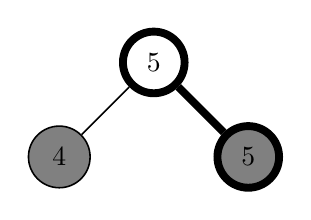
\begin{tikzpicture}[bold, scale=12]
                % The Tree
                \node(0)[max]{5}
                child{node [min, thin]{4} edge from parent[thin]}
                child{node [min]{5}};
            \end{tikzpicture}
        }
    \end{subfigure}
    &
    \begin{subfigure}[b]{0.22\textwidth}
        \centering
        \resizebox{\textwidth}{!}{
            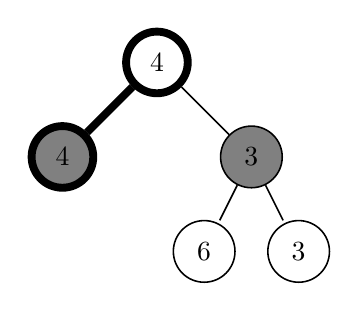
\begin{tikzpicture}[bold, scale=12]
                % The Tree
                \node(0)[max]{4}
                child{node [min]{4}}
                child{node [min, thin]{3}
                    child{node [max] {6}}
                    child{node [max] {3}}
                    edge from parent[thin]
                };
            \end{tikzpicture}
        }
    \end{subfigure}
    &
    \begin{subfigure}[b]{0.22\textwidth}
        \centering
        \resizebox{\textwidth}{!}{
            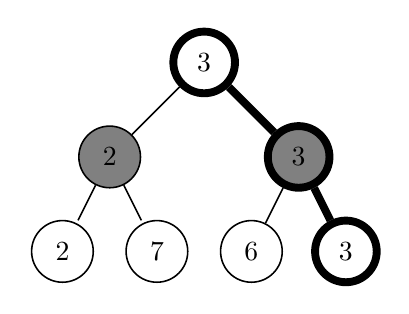
\begin{tikzpicture}[bold, scale=12]
                % The Tree
                \node(0)[max]{3}
                child{node [min, thin]{2}
                    child{node [max] {2}}
                    child{node [max] {7}}
                    edge from parent[thin]
                }
                child{node [min]{3}
                    child{node [max, thin] {6}
                        edge from parent [thin]
                    }
                    child{node [max] {3}}
                };
            \end{tikzpicture}
        }
    \end{subfigure}
    &
    \begin{subfigure}[b]{0.22\textwidth}
        \centering
        \resizebox{\textwidth}{!}{
            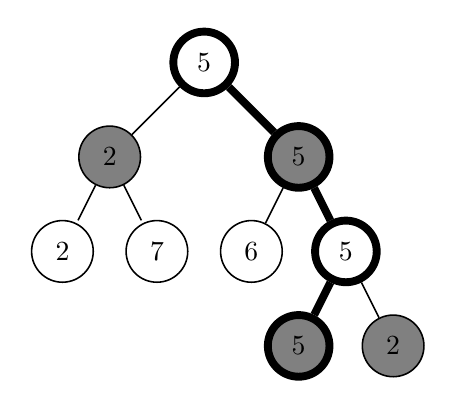
\begin{tikzpicture}[bold, scale=12]
                % The Tree
                \node(0)[max]{5}
                child{node [min, thin]{2}
                    child{node [max] {2}}
                    child{node [max] {7}}
                    edge from parent[thin]
                }
                child{node [min]{5}
                    child{node [max, thin] {6}
                        edge from parent [thin]
                    }
                    child{node [max] {5}
                        child{node [min] {5}}
                        child{node [min, thin] {2}
                            edge from parent [thin]
                        }
                    }
                };
            \end{tikzpicture}
        }
    \end{subfigure}

    \end{tabular}

    \caption{Best first minimax on an example tree. Each iteration expands
    all children of the leaf at the end of the principal variation, and
    backpropagates the new minimax values up the tree.}

    \label{fig:bestfirstminimax}

\end{figure}
